\documentclass[11pt,a4paper]{article}

\usepackage[polish]{babel}
\usepackage{polski}
\usepackage[utf8]{inputenc}
\usepackage[T1]{fontenc}
\usepackage{graphicx}
\usepackage{color}
\usepackage{placeins}
\usepackage[math]{anttor}
\usepackage{natbib}
\usepackage{url}
\frenchspacing

\newcommand{\todo}[1]{\colorbox{yellow}{#1}}

\begin{document}

\title{Automatyczna klasyfikacja i ekstrakcja tematu krótkich notatek w języku polskim}
\author{Paweł Obrok\\pod kierunkiem dr. Michała Korzyckiego}

\maketitle
\pagebreak

\tableofcontents
\pagebreak

\section{Wstęp}
\section{Podstawy teoretyczne}
\section{Procedura badawcza}

Do badań wykorzystano pakiet gensim \cite{gensim}. Jest to biblioteka napisana
w języku Python tworzoan przez Radima Řehůřeka i stawiająca sobie za cel
udostępnienie narzędzi do łatwego i wydajnego przetwarzania tesktów w językach
naturalych. Zawiera ona szereg funkcjonalności użytecznych w zadaniach
dotyczących przetwarzania języka naturalnego takich jak:

\begin{itemize}
\item Implementacje algorytmów LDA i LSI wraz z wersjami roproszonymi
\item Implementacje kilku popularnych schematów wagowych (patrz \ref{weighting})
\item Zarządzanie korpusami tekstów i obsługa formatów stosowanych przez SVMlight \cite{svmlight},
LDA-C \cite{lda-c} i GibbsLDA++ \cite{gibbs-lda}
\item Wydajne obliczanie podobieństwa między dokumentami w sensie danego modelu
\item Wyszukiwanie kolokacji
\end{itemize}

Algorytm stosowany w pakiecie gensim do estymacji parametrów LDA opisany jest
w pełni w \cite{gensim-algorithm}.

\subsection{Słownik fleksyjny}

Do sprowadzenia wyrazów występujących w tekście do form podstawowych
zastosowany został słownik fleksyjny języka polskiego CLP
\cite{gajecki-slownik} rozwijany w Zespole Przetwarzania Języka Naturalnego
Instytutu Informatyki AGH. Jest to biblioteka napisana w języku C,
udostępniająca interfejs pozwalający przeszukiwać zawarte w słowniku dane.
Słownik obejmuje obecnie ponad 150 tysięcy wpisów co pokrywa niemal całkowicie
zbiór polskich wyrazów pospolitych. Zawiera on także najczęściej występujące
nazwy własne i skróty.

CLP oferuje następujące funkcjonalności:
\begin{enumerate}
\item Zwrócenie listy możliwych form podstawowych dla danego wyrazu
\item Zwrócenie etykiety fleksyjnej, w której zawarty jest sposób odmiany
danej formy podstawowej
\item Znalezienie dla danego wyrazu wektora odmiany opisującego formę
w jakiej występuje
\end{enumerate}

Przykładowo, dla wyrazu ``zamek'' uzyskać można następujące informacje:

\begin{quote}
ID: 286975056\\
Forma podstawowa: zamek\\
Formy: zamek, zamka, zamkowi, zamkiem, zamku, zamki, zamków, zamkom, zamkami,
zamkach\\
Etykieta: ACABBA\\
Opis etykiety: rzeczownik / męski nieżyw. / M.Lp.-0 / M.Lm.-i / D.Lp.-a /
D.Lm.-ów\\
Wektor odmiany: [1, 4]\\
\end{quote}

\begin{quote}
ID: 286975040\\
Forma podstawowa: zamek\\
Formy: zamek, zamku, zamkowi, zamkiem, zamki, zamków, zamkom, zamkami,
zamkach\\
Etykieta: ACABA\\
Opis etykiety: rzeczownik / męski nieżyw. / M.Lp.-0 / M.Lm.-i / D.Lp.-u\\
Wektor odmiany: [1, 4]\\
\end{quote}

\subsection{Preprocessing}

Aby zmniejszyć rozmiar przetwarzanych danych i poprawić ich uwarukowanie po
sprowadzeniu wszystkich wyrazów danego dokumentu do form podstawowych
zastosowano dodatkowy preprocessing polegający na odrzuceniu wyrazów
występujących w więcej niż 70\% dokumentów i takich, które wystąpiły w co
najwyżej jednym dokumencie. Te pierwsze nie niosą żadnej informacji o rodzaju
tekstu, w którym występują ze względu na swoją pospolitość. Powiązania tych
drugich nie mogłyby być wychwycone przez algorytmy redukcji wymiaru macierzy.

Zastosowano również kilka innych prostych operacji, jak na przykład
zamienienie wszystkich liczb na token ``NUMBER'' a wyrażeń typ ``2:3''
na token ``RATIO''.

Przykładowo następujący dokument:

\begin{quote}
\#000064\\
Drużyna Krzysztofa Oliwy - New Jersey Devils, mająca najlepszy 
bilans w całej NHL, odniosła kolejne zwycięstwo, pokonując w 
środę na własnym lodowisku New York Rangers 4:1. 
\end{quote}

po poddaniu preprocessingowi przyjmie postać:

\begin{quote}
NUMBER\\
drużyna Krzysztof oliwa - new jersey devils , mający najlepszy bilans
cały NHL , odnieść kolejny zwycięstwo , pokonując środa własny lodowisko new
York rangers RATIO 
\end{quote}

\subsection{Dobór schematu wagowego}
\label{weighting}

Bezpośrednie zastosowanie podejścia bag-of-words może dawać mylny obraz
dokumentu --- pewne wyrazy mogą pojawiać się bardzo często a mimo to nie
dostarczać żadnej pożytecznej informacji o danym dokumencie ze względu na fakt
występowania bardzo często w danym korpusie. Innym problemem może być
przecenianie wielokrotnego występowania danego wyrazu --- trzykrotne pojawienie
się pewnego wyrazu raczej nie sugeruje trzykrotnie większego prawdopodobieństa,
że jest on kluczowy dla tekstu. Aby rozwiązać pierwszy z tych problemów stosuje
się normalizowanie wag wyrazów w danym dokumencie przez jakiś współczynnik
charakteryzujący częstość występowania tego wyrazu w całym korpusie. Drugi z
nich można rozwiązać przez zastosowanie funkcji typu logarytm czy pierwiastek.
Dokładny dobór zastosowanych na tym etapie przekształceń nazywamy schematem
wagowym.

W tej pracy zastosowano schemat wagowy nazywany ''Log Entropy``.  Intuicyjnie
polega on na wykorzystaniu ilości informacji w sensie Shannona niesionej przez
dany wyraz jako czynnika normalizacyjnego (dla często spotykanych wyrazów
będzie on niski) i zastosowaniu logarytmu jako funkcji wygładzającej.

Mając daną macierz $w_{ij}$, której $j$-ty wiersz odpowiada $j$-temu
dokumentowi, a jego $i$-ta pozycja zawiera liczbę wystąpień $i$-tego wyrazu w
tym dokumecie dokonujemy przeształcenia opisanego równaniami
\ref{eq:log-entr-beg}--\ref{eq:log-entr-end} uzyskując macierz $a_{ij}$
zawierającą nowe wagi wyrazów.

\begin{equation}
  \label{eq:log-entr-beg}
  p_{ij} = \frac{tf_{ij}}{gf_i}
\end{equation}

\begin{equation}
  g_i = 1 + \sum_{j=1}^n \frac{p_{ij} log(p_{ij})}{log(n)}
  \todo{$log(p_{ij}) = -\infty?$}
\end{equation}

\begin{equation}
  \label{eq:log-entr-end}
  a_{ij} = g_i log(tf_{ij} + 1)
\end{equation}

Drobiazgowe omówienie i porównanie różnych schematów wagowych znaleźć moż\-na w
\cite{figiel}.

\subsection{Przetwarzanie zapytania}
\label{processing}
\todo{Transformacja do przestrzeni topicow}

Mając dany model macierzowy dla pewnego korpusu pojawia się standardowy problem
wykonania zapytania do modelu i uzyskania z niego informacji. Dla pewnego
dokumentu stanowiącego zapytanie $d_q$ (może to być dokument, podobny do tych,
które znajdują się w korpusie, albo po prostu zbitek wyrazów w rodzaju zapytań
wprowadzanych zwykle w wyszukiwarce internetowej) chcielibyśmy uzyskać teksty z
korpusu $d_i$ posortowane według malejącej oceny podobieństwa tych tekstów do
$d_q$. W tym celu obliczamy dla każdego $d_i$ ranking $r_i$ według wzorów
\ref{similarity-computation-beg}-\ref{similarity-computation-end}.

\begin{equation}
\label{similarity-computation-beg}
  \langle d_i, d_j \rangle = \sum_k^n d_{ik}d_{jk}
\end{equation}

\begin{equation}
  ||d|| = \langle d, d \rangle
\end{equation}

\begin{equation}
  \label{similarity-computation-end}
  r_i = cos(d_i, d_j) = \langle \frac{d_i}{||d_i||}, \frac{d_j}{||d_j||} \rangle
\end{equation}

Nietrudno zauważyć, że obliczone rankingi to po prostu odległość kosinusowa
między wektorami reprezentującymi dokumenty.  Warto zauważyć, że same rankingi
$r_i$ także mogą okazać się przydatne, gdyż zawierając informację o ocenie
stopnia podobieństwa między dokumentami przez system. Można sobie wyobrazić
sytuację, w której na ich podstawie obliczan i wyświetlane operatorowi będzie
prawdopodobieństow, że dany dokument jest tym, czego szuka.

\subsection{Obliczanie perplexity}

Współczynnik perplexity który zaproponowany był do oceny modeli języka
\cite{bahl-perplexity} a oddawać niejako poziom ``zaskoczenia'' modelu
niewidzianymi dotąd danymi. Jest on tak dobrany, że rzut symetryczną,
$k$-ścienną kością będzie miał perplexity dokładnie $k$ - możemy co najwyżej
przewidywać, że nastąpi jeden z $k$ rezultatów. Można też zdefiniować go jako
eksponentę z entropii. Oczywiście jeżeli współczynnik ten się zmniejsza, to
można powiedzieć, że model lepiej opisuje dane zjawisko.

Jeżeli $p_i$ to prawdopodobieństwo przypisywane przez nasz model zdarzeniu
polegającemu na wygenerowaniu $i$-tego wyrazu w danym dokumencie, znając temat
lub tematy i ich wagi przyporządkowane danemu dokumentowi przez system, to
znormalizowany współczynnik perplexity dla tego wyrazu opisany jest wzorem
\ref{perplexity}.

\begin{equation}
  \label{perplexity}
  \frac{2^{-\sum_{i/1}^n p_ilog_2(p_i)}}{n}
\end{equation}

Aby obliczyć prawdopodobieństwo $p_i$ obliczamy odległość kosinusową $d_i$
między danym wyrazem, a dokumentem, zgodnie z \ref{processing}. Następnie
dokonujemy transformacji \ref{to-probability}, gdzie $d_j$ to odległość
kosinusowa $j$-tego wyrazu rozponawanego przez system od danego dokumentu.

\begin{equation}
  \label{to-probability}
  p_i = \frac{\pi - arccos(d_i)}{\sum_j^N \pi - arccos(d_j)}
\end{equation}

\section{Opis danych}

Działanie algorytmów LDA i LSI analizowane było na zbiorze około 50000 notatek
Polskiej Agencji Prasowej. Notatki te to krótkie wiadomości tekstowe, z których
większość dotyczy pojedynczego wydarzenia. Dotyczą one różnych dziedzin życia,
co nadaje temu zbiorowi dodatkową różnorodność i pozwala oczekiwać, że
osiągnięte wyniki będą miarodajne dla efektywności algorytmów w prawdziwych
zastosowaniach.

\subsection{Przykładowy problem}
\label{sec:example}

Aby przetestować działanie obu algorytmów przygotowane zostało przykładowe
zapytanie do systemu wyszukiwania informacji dla zbioru notatek prasowych PAP.
Problem polega na znalezieniu dokumentów podobnych do pojedynczej wybranej
notatki na temat bliźniaczek syjamski. Została przygotowana modelowa odpowiedź
systemu dla porównania z faktycznymi odpowiedziami.

Zapytanie:

\begin{quote} ***** \#000424 *****\\ W sobotę polskie bliźniaczki syjamskie
Weronika i Wiktoria przylecą do Polski rejsem Newark-Kraków - poinformował PAP
oddział LOT-u na nowojorskim lotnisku.  Bliźniaczki syjamskie Weronika i
Wiktora urodziły się 26 maja 1999 w szpitalu Akademii Medycznej w Lublinie. Od
16 sierpnia przebywają w Filadelfii. W listopadzie przeszły udaną operację
rozdzielenia. Pierwszy termin wypisania dziewczynek wyznaczono na 11 lutego.
Został jednak przesunięty o tydzień z uwagi na gorączkę Weroniki.  \end{quote}

Najbardziej podobne dokumenty wybrane ręcznie:

\begin{quote} ***** \#000516 *****\\ Wiktoria i Weronika, siostry syjamskie
rozdzielone w listopadzie w Filadelfii, przyleciały z mamą w sobotę rano do
Krakowa. Na lotnisku w Balicach żonę i córki przywitał ojciec dziewczynek,
Edward Paleń. Byli też trzej bracia dziewczynek.  "Dziewczynki przyjechały w
dobrym stanie, są zdrowe" - powiedziała na lotnisku w Balicach mama
rozdzielonych bliźniaczek pani Krystyna Paleń. "Lekarze amerykańscy twierdzili,
że gdyby dziewczynki miały po powrocie do kraju trafić do polskiego szpitala,
to oni by je przytrzymali dłużej u siebie. Wypisali dziewczynki w takim stanie,
że mogą iść do domu" - powiedziała dziennikarzom. Dodała, że Wiktoria i
Weronika będą znajdowały się pod opieką lekarza pediatry w Stalowej Woli.
\end{quote}

\begin{quote} ***** \#009928 *****\\ W klasztorze Ojców Kapucynów w Stalowej Woli
(Podkarpacie) ochrzczone zostały w niedzielę syjamskie bliźniaczki - Weronika i
Wiktora Paleniówny, które urodziły się 26 maja ub. roku częściowo zrośnięte
klatkami piersiowymi i brzuszkami. Pomoc w rozdzieleniu dzieci zaoferował
Szpital Dziecięcy w Filadelfii w USA.  Rozdzielenia dokonano 3 listopada, po
kilkunastogodzinnej operacji, w której udział wzięło 45 lekarzy.  \end{quote}

\begin{quote} ***** \#011189 *****\\ Powoli stabilizuje się stan zdrowia
9-miesięcznego Kamila, jednego z rozdzielonych w Krakowie braci syjamskich.
Drugi z braci - Patryk - nadal jest w ciężkim stanie - poinformował w
poniedziałek PAP opiekujący się braćmi docent Adam Bysiek.  Stan zdrowia Kamila
docent Bysiek określił jako "rokujący nadzieję". Obaj bracia nadal przebywają
na oddziale intensywnej terapii Polsko-Amerykańskiego Instytutu Pediatrii
Uniwersytetu Jagiellońskiego w Krakowie Prokocimiu.  Bracia zostali rozdzieleni
tydzień temu. O terminie operacji zadecydowało nagłe pogorszenie się stanu
zdrowia jednego z nich.  Początkowo operacja rozdzielenia była planowana na
wrzesień. Na początku czerwca braciom wszczepiono ekspandery, mające za zadanie
namnożyć tkankę skórną potrzebną po operacji.  Operacja trwała 8 godzin,
uczestniczyło w niej 14 lekarzy oraz zespół anestezjologów i pielęgniarek. Jej
pierwszą część zajęło rozdzielenie braci, w drugiej lekarze zajęli się
rekonstrukcją rozdzielonych narządów. Bracia byli zrośnięci powłokami
piersiowo-brzusznymi, mieli wspólną przeponę, worek osierdziowy i wątrobę.
Była to siódma operacja rozdzielenia bliźniaków syjamskich dokonana w
Instytucie w Prokocimiu.  \end{quote}

\begin{quote} ***** \#008779 *****\\ Bracia syjamscy Kamil i Patryk przeszli w
poniedziałek pierwszy zabieg przygotowujący ich do operacji rozdzielenia,
planowanej za trzy miesiące w Polsko-Amerykańskim  Instytucie Pediatrii UJ w
Krakowie-Prokocimiu.  \end{quote}

\begin{quote} ***** \#005662 *****\\ W Polsko-Amerykańskim Instytucie Pediatrii w
Krakowie-Prokocimiu zmarły siostry syjamskie, które urodziły się przed
tygodniem w Wejherowie.  \end{quote}

\begin{quote} ***** \#000469 *****\\ Bliźniaczki syjamskie z Poznania - Małgosia i
Dorota - przeszły już pierwsze badania w Polsko-Amerykańskim Instytucie
Pediatrii UJ w Krakowie-Prokocimiu." Z przeprowadzonych badań wynika, że
siostry mają wspólną watrobę i przeponę oraz prawdopodobnie wspólne drogi
żółciowe i serce" - powiedział PAP opiekujący się bliźniaczkami dr Adam Bysiek
z Instytutu. Siostry urodziły się 11 lutego w poznańskiej klinice św. Rodziny.
Dziewczynki zrośnięte są brzuszkami i klatkami piersiowymi.  \end{quote}

\begin{quote} ***** \#005855 *****\\ Liczba urodzeń bliźniąt syjamskich nie
odbiega w Polsce od statystycznej normy - powiedział PAP prof. Jan Grochowski,
dyrektor Polsko-Amerykańskiego Instytutu Pediatrii UJ, w którym przebywają dwie
pary bliźniąt syjamskich.  \end{quote}

\begin{quote} ***** \#010677 *****\\ Lekarze z Polsko-Amerykańskiego Instytutu
Pediatrii UJ w Krakowie Prokocimiu rozdzielili 9-miesięcznych braci syjamskich
Kamila i Patryka - poinformował PAP doc. Adam Bysiek, szef zespołu opiekującego
się bliźniętami.  \end{quote}

\begin{quote} ***** \#007320 *****\\ Prof. Louis Gerald Keith, który w ubiegłym
roku przeprowadził operację rozdzielenia polskich bliźniaczek syjamskich
Weroniki i Wiktorii, został odznaczony przez prezydenta Aleksandra
Kwaśniewskiego Krzyżem Oficerskim Zasługi RP.  \end{quote}

\begin{quote} ***** \#007872 *****\\ Komitet etyki szpitala w Palermo na Sycylii
wydał zgodę na operację peruwiańskich bliźniaczek syjamskich, w wyniku której
jedna z nich ma szansę na ocalenie kosztem życia drugiej - doniosła prasa
włoska.  \end{quote}

\begin{quote} ***** \#012193 *****\\ Jeden z 9-miesięcznych braci syjamskich,
rozdzielonych przez lekarzy w Krakowie pod koniec czerwca, zmarł w środę
wieczorem z powodu niewydolności krążenia - poinformował PAP docent Adam
Bysiek.  \end{quote}

\section{Wyniki i analiza}

Niniejszy rozdział zawiera porównanie różnych aspektów działania algorytmów LDA
i LSI. Na jego końcu znajdują się wnioski jakie można wyciągnąć z zebranych
danych.

\subsection{Tematy}

Tabele \ref{fig:lsi_topics} i \ref{fig:lda_topics} zawierają niektóre tematy
wygenerowane przez algorytmy LSI i LDA skonfigurowane na 100 tematów (po
dziesięć najbardziej znaczących słów w każdym temacie). Pojedynczy wiersz
tabeli zawiera jeden temat - liczby przy tokenach oznaczają wagi poszczególnych
słów w danym temacie.

Tematy uzyskane przy pomocy LDA wydają się bardziej odpowiadać postrzeganiu
tekstu przez człowieka niż te wygenerowane przez LSI.  Przykładowo temat numer 4 w tabeli
\ref{fig:lsi_topics} można interpretować jako ,,nie pogoda i finanse`` ---
możliwość złożenia dwóch tematów postrzeganych przez człowieka w jeden, ale z
przeciwnymi znakami powoduje powstawanie tego typu kombinacji. Tematy wygenerowane
przez LDA bywają złożeniami dwóch różnych konceptów, jednak zawsze mają ten sam znak,
jak na przykład temat numer 5 w tabeli \ref{fig:lda_topics}, który wydaje się łączyć
koncepty ,,muzeum`` i ,,przestępstwo``.

\begin{table}[h]
\label{fig:lsi_topics}
\caption{Tematy wyekstrahowane przez algorytm LSI}
\begin{tabular}{|c|p{\linewidth}|}
\hline
Lp. & Temat \\\hline
1 & 0.269*" + 0.181*- + 0.171*być + 0.161*procent + 0.144*polski + 0.138*rok + 0.119*) + 0.118*złoty + 0.111*( + 0.102*a \\\hline
2 & -0.304*procent + -0.265*wzróść + -0.254*punkt + -0.211*WIG + -0.192*wynieść + -0.191*spaść + -0.180*złoty + -0.165*spółka + -0.158*akcja + 0.158*" \\\hline
3 & 0.482*RATIO + 0.265*mecz + 0.234*: + 0.187*pokonać + 0.182*mistrzostwo + 0.149*) + 0.149*turniej + -0.142*" + 0.119*piłkarski + 0.117*wygrać \\\hline
4 & -0.301*stopień + -0.250*temperatura + -0.240*maksymalny + -0.228*wiatr + -0.222*umiarkowany + -0.216*deszcz + -0.212*słaby + -0.208*opad + -0.181*południe + 0.164*złoty \\\hline
5 & -0.390*złoty + -0.305*grosz + -0.262*dolar + -0.246*euro + 0.210*punkt + -0.195*osiągać + -0.170*milion + 0.159*WIG + -0.147*umocnić + 0.142*procent \\\hline
6 & -0.355*spółka + -0.301*Akcyjna + 0.259*grosz + -0.223*milion + 0.215*zamknięcie + 0.185*euro + 0.180*osiągać + 0.170*punkt + 0.153*dolar + -0.148*bank \\\hline
7 & -0.435*procent + 0.300*spółka + -0.232*rok + 0.212*akcja + -0.191*proca + 0.190*Akcyjna + 0.148*giełda + -0.133*milion + 0.127*zmienić + 0.124*kurs \\\hline
8 & -0.227*RATIO + 0.192*sąd + -0.147*: + 0.147*( + -0.135*unia + -0.129*mecz + 0.127*policja + -0.125*spółka + 0.122*tysiąc + -0.122*AWS \\\hline
9 & 0.313*( + 0.274*) + -0.258*RATIO + -0.165*mecz + -0.158*sąd + -0.144*: + 0.133*wyścig + 0.126*mistrzostwo + 0.120*spółka + 0.120*świat \\\hline
10 & -0.230*sąd + 0.220*europejski + -0.187*AWS + 0.154*unia + -0.148*procent + 0.143*UE + -0.119*wyborczy + -0.118*okręgowy + 0.114*polski + 0.111*milion \\\hline
\end{tabular}
\end{table}

\begin{table}[h]
\label{fig:lda_topics}
\caption{Tematy wyekstrahowane przez algorytm LDA}
\begin{tabular}{|c|p{\linewidth}|}
\hline
Lp. & Temat \\\hline
1 & 0.027*open + 0.026*powodzianin + 0.021*podlaski + 0.018*Słowenia + 0.017*cukrownia + 0.017*najstarszy + 0.013*przedstawiony + 0.012*urodziny + 0.012*rata + 0.012*zrezygnować\\\hline
2 & 0.021*europejski + 0.021*unia + 0.018*UE + 0.012*polski + 0.011*kraj + 0.010*" + 0.009*Litwa + 0.009*unijny + 0.008*państwo + 0.008*NATO\\\hline
3 & 0.032*palestyński + 0.031*Izrael + 0.030*izraelski + 0.023*Palestyńczyk + 0.015*Arafat + 0.013*szaron + 0.013*świętokrzyski + 0.012*zawieszenie + 0.012*autonomia + 0.011*arabski\\\hline
4 & 0.024*sąd + 0.015*aresztować + 0.015*podejrzany + 0.014*rejonowy + 0.013*okręgowy + 0.013*śledczy + 0.013*akt + 0.012*Gdynia + 0.012*oskarżenie + 0.012*Radom\\\hline
5 & 0.016*wierzyciel + 0.013*muzeum + 0.013*wystawa + 0.011*zbiór + 0.011*śląski + 0.011*Brazylijczyk + 0.010*łączny + 0.010*zajmujący + 0.009*przestępczy + 0.009*łódzki\\\hline
6 & 0.032*festiwal + 0.022*woj + 0.017*Białystok + 0.017*letni + 0.014*wielkopolski + 0.014*wrzesień + 0.014*kupno + 0.012*ogólnopolski + 0.012*usuwanie + 0.012*impreza\\\hline
7 & 0.019*siatkarz + 0.011*obniżka + 0.009*noc + 0.007*postać + 0.006*Gorzów + 0.006*artystyczny + 0.006*bóg + 0.006*bandyta + 0.005*nieznany + 0.005*ZSRR\\\hline
8 & 0.012*" + 0.011*general + 0.010*motors + 0.008*Jedwabne + 0.008*kardynał + 0.007*film + 0.007*weekend + 0.007*Józef + 0.007*rocznica + 0.006*odbyć\\\hline
9 & 0.017*świat + 0.016*klasa + 0.016*TP + 0.015*metr + 0.015*( + 0.015*) + 0.014*mistrzostwo + 0.014*zająć + 0.013*AZS + 0.013*bieg\\\hline
10 & 0.044*obligacja + 0.021*Artur + 0.018*włosek + 0.017*pomnik + 0.016*politechnika + 0.016*białostocki + 0.016*społeczność + 0.013*wyeliminować + 0.012*skorzystać + 0.011*wyemitować\\\hline
\end{tabular}
\end{table}

\FloatBarrier

\subsection{Czas działania}

\todo{Czy to ma sens?}

\subsection{Metryki z nadzorem}

W tym rozdziale omówiono wyniki otrzymane za pomocą algorytmów LDA i LSI dla
przykładowego problemu opisanego w \ref{sec:example}. Należy zauważyć, że tego
rodzaju ewaluacja wymaga ręcznego przygotowania danych testowych przez
człowieka, co może być nieprakyczne dla dużych zbiorów danych.  Jej zaletą jest
fakt, że mierzy ona faktyczne osiągi danego rozwiązania w rzeczywistych
problemach.

\subsubsection{Ranking dokumentów}

Wykresy \ref{ranks_stemming_comparison} i \ref{ranks_no_stemming_comparison}
przedstawiają sumę kwadratów ranków dokumentów z wzorca przygotowanego ręcznie
dla danego zapytania w wynikach działania odpowiednio algorytmów LDA i LSI dla
różnej liczby tematów.

Algorytm LDA osiąga ogólnie gorsze wyniki niż LSI - poza przedziałem $50 - 100$
tematów. Gorszy jest też (aczkolwiek niewiele) najlepszy wynik jaki udałoby się
osiągnąć odpowiednio dobierając liczbę tematów. Na wykresie daje się także
zauważyć stochastyczna natura LDA - podczas gdy dla LSI wyniki niemal
monotonicznie poprawiają się wraz ze wzrostem liczby tematów dla LDA zdarza się
znaczne pogorszenie wyników przy zwiększeniu tej liczby.

Polepszenie wyników dzięki zastosowaniu stemmingu jest widoczne na pierwszy
rzut oka --- polski jako język silnie fleksyjny jest znakomitym kandydatem do
zastosowania tego typu techniki. W \cite{manning-schuetze} zasugerowano, że ze
stemmingu można zrezygnować dyponując odpowiednio dużym zbiorem danych jednak
wyniki te uzyskano dla języka angielskiego, którego fleksja jest znacznie mniej
rozbudowana. W tym wypadku zebranie tak dużej ilości danych może być mniej
praktyczne niż skonstruowanie słownika fleksyjnego takiego jak na przykład ten
opisany w \cite{pisarek-slownik}.

Co ciekawe algorytm LDA radzi sobie znacznie lepiej od LSI bez wykorzystania
stemmingu.  Może to być spowodowane trudnością w przypadku LSI połączenia ze
sobą słów, które różnią się formą fleksyjną i są w tym wypadku traktownae
całkowicie osobno.

\begin{figure}[h]
\caption{Suma kwadratów ranków dokumentów ze wzorca dla testowego zapytania (z wykorzystaniem stemmingu)}
\label{ranks_stemming_comparison}
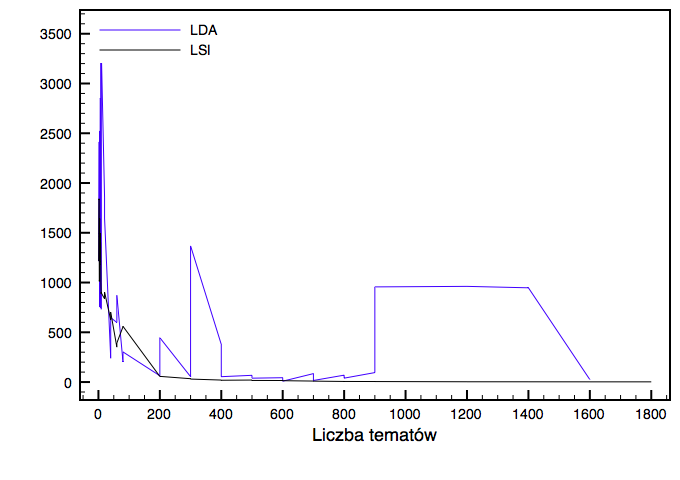
\includegraphics[width=\linewidth]{gfx/ranks_stemming.png}

\caption{Suma kwadratów ranków dokumentów ze wzorca dla testowego zapytania (bez wykorzystania stemmingu)}
\label{ranks_no_stemming_comparison}
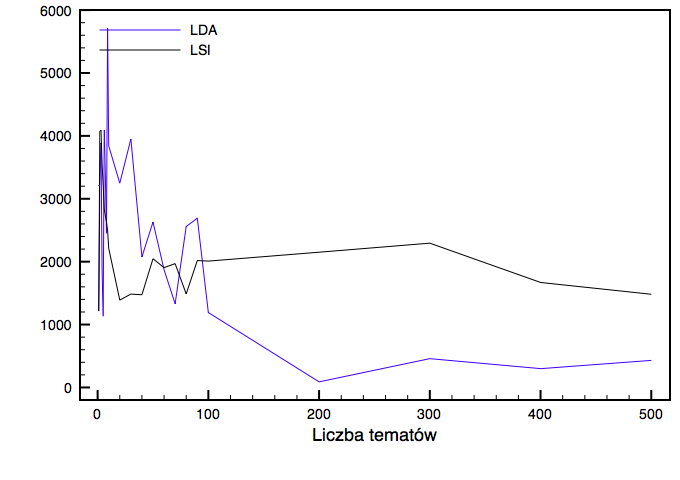
\includegraphics[width=\linewidth]{gfx/ranks_no_stemming.png}
\end{figure}

\FloatBarrier

\subsubsection{Krzywe ROC}

Krzywa ROC \cite{roc-article1} (Receiver Operation Characteristic) to wykres
przedstawiający dla danego klasyfikatora zależność między stosunkiem liczby
znalezionych dokumentów relewantnych do liczby wszystkich zwróconych dokumentów
(TPR --- True Positive Rate), a stosunkiem liczby odrzuconych dokumentów
relewantnych do liczby wszystkich odrzuconych dokumentów (FPR - False Positive
Rate) w miarę zmiany progu detekcji. W tym wypadku ten zmienny próg to po
prostu liczba $n$ - pierwszych $n$ dokumentów jest traktowane jako odnalezione,
a pozostałe jako odrzucone.

Lepsze klasyfikatory charakteryzują się krzywymi ROC położonymi dalej od linii
$x = y$.  Klasyfikatory blisko, lub na tej linii nie wykonują żadnej użytecznej
pracy. Analiza odległości krzywej ROC od linii $x = y$ w różnych miejscach
wykresu może dać wskazówkę co do najlepszego dobrania progu detekcji dla danego
problemu.

Wykresy \ref{roc_lsi} i \ref{roc_lda} przedstawiają krzywe ROC dla algorytmów
LDA i LSI dla różnych liczb tematów. Dla dużych liczb tematów algorytm LDA
spisuje się gorzej, jednak można zauważyć, że klasyfikator uzyskany dla 30
tematów jest podobnej jakości lub lepszy jak ten uzyskany przy użyciu LSI dla
100 tematów.

\begin{figure}[h]
\caption{Krzywe ROC dla algorytmu LSI dla wybranych liczb tematów}
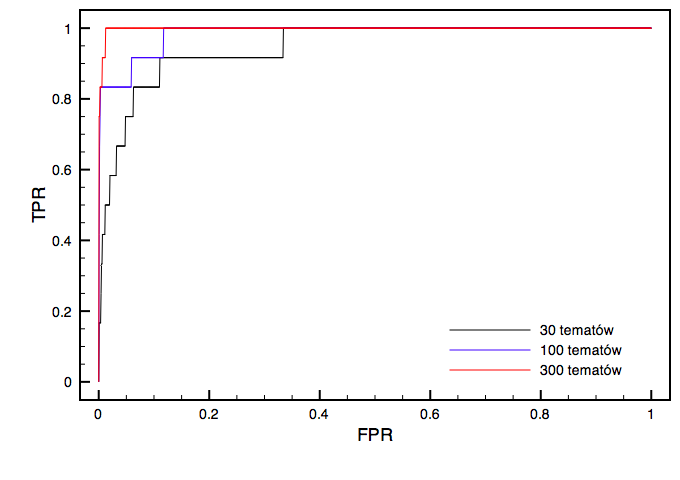
\includegraphics[width=\linewidth]{gfx/lsi_roc.png}
\label{roc_lsi}

\caption{Krzywe ROC dla algorytmu LDA dla wybranych liczb tematów}
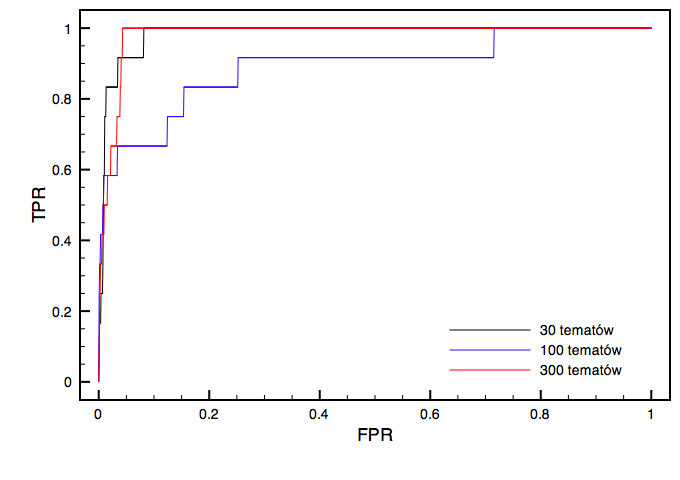
\includegraphics[width=\linewidth]{gfx/lda_roc.png}
\label{roc_lda}
\end{figure}

Na wykresach \ref{roc_lsi_untagged} i \ref{roc_lda_untagged} przedstawione
zostały krzywe ROC dla algorytmów LSI i LDA bez wykorzystania stemmingu.
Ponownie daje się zauważyć lepsze działanie algorytmu LDA w tym wypadku -
klasyfikator uzyskany dla 300 tematów jest znacznie lepszy od tego uzyskanego
przy pomocy LSI.

\begin{figure}[h]
\caption{Krzywe ROC dla algorytmu LSI dla wybranych liczb tematów bez wykorzystania stemmingu}
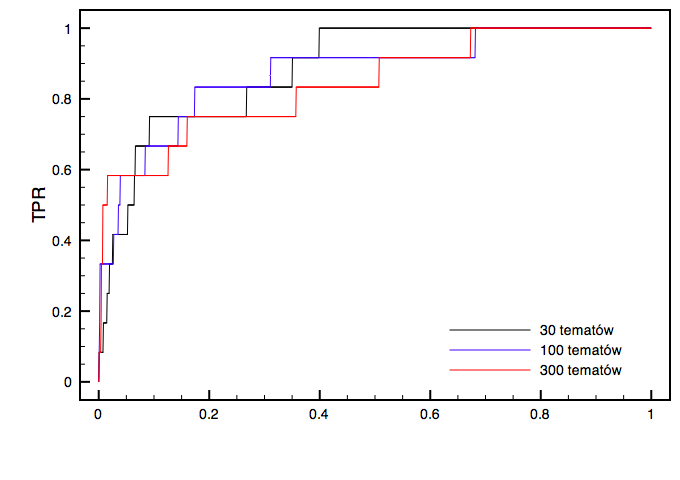
\includegraphics[width=\linewidth]{gfx/lsi_roc_untagged.png}
\label{roc_lsi_untagged}

\caption{Krzywe ROC dla algorytmu LDA dla wybranych liczb tematów bez wykorzystania stemmingu}
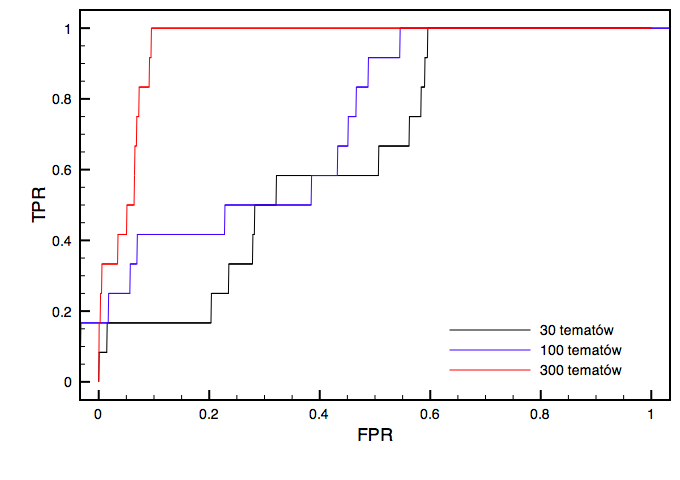
\includegraphics[width=\linewidth]{gfx/lda_roc_untagged.png}
\label{roc_lda_untagged}
\end{figure}

\FloatBarrier

\subsubsection{Przywołanie i precyzja}

Przywołanie (stosunek liczby zwróconych relewantnych dokumentów do liczby
wszystkich relewantncyh dokumentów) i prezycja (stosunek liczby zwróconych
relewantncyh dokumentów do liczby wszystkich zwróconych dokumentów) to częste
metryki w zadaniach typu information retrieval. Wybranie jakiegoś poziomu
przywołania reprezentuje pewien kompromis między kompletnością zwróconych
danych, a częstością występowania w nich danych relewantnych, a więc ilością
czasu, które musi poświęcić operator systemu na ich dalsze przetworzenie.

Wykresy \ref{fig:lsi_precision} i \ref{fig:lda_precision} prezentują precyzę
osiąganą przez algorytmy LDA i LSI na różnych poziomach przywołania dla
przykładowego problemu.

Można zauważyć, że LDA daje znacznie gorszą precyzję niż LSI. Nawet najlepiej
dobrana liczba tematów (w tym wypadku 300) pozwala osiągać precyzję
porównywalną jedynie z LSI dla 30 tematów.

\begin{figure}[h]
\caption{Precyzja na różnych poziomach przywołania dla algorytmu LSI}
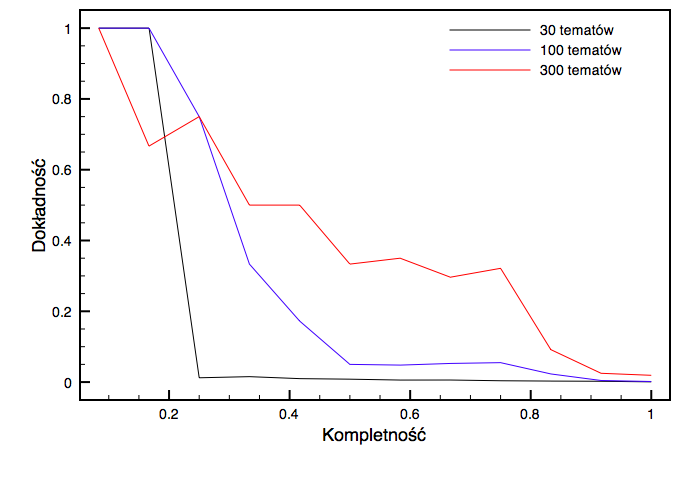
\includegraphics[width=\linewidth]{gfx/lsi_precision.png}
\label{fig:lsi_precision}
\end{figure}

\begin{figure}[h]
\caption{Precyzja na różnych poziomach przywołania dla algorytmu LDA}
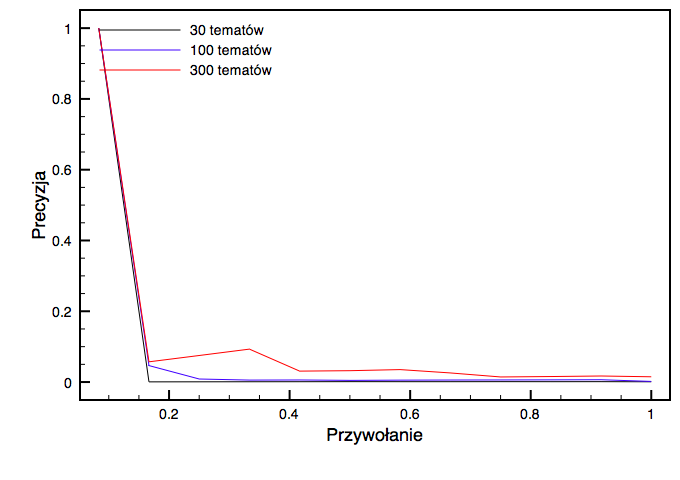
\includegraphics[width=\linewidth]{gfx/lda_precision.png}
\label{fig:lda_precision}
\end{figure}

\FloatBarrier

\subsection{Metryki bez nadzoru (perplexity)}

Współczynnik perplexity, którego wartości w zależności od liczby tematów są
przedstawione na wykresie \ref{fig:perplexity}, daje pewne pojęcie o tym jak
dobrze model jest w stanie przewidzieć nowe dane. Wysokie wartości
współczynnika mogą wskazywać, że model jest przeuczony i będze słabo uogólniał
swoje działania na nieznane dane. Jest on dobrym wskaźnikiem jak dobrze dany
model będzie sobie radził z klastrowaniem danego zbioru danych.

Wykres demonstruje, że optymalne wartości współczynnika perplexity zostają
osiągnięte w okolicach 50 tematów. W tym wypadku może to sugerować, że mniej
więcej na tyle właśnie grup tematycznych należałoby podzielić ten zbiór danych.

Algorytm LDA zachowuje niski współczynnik perplexity tylko stosunkowo blisko
optymalnej liczby tematów. Takie zachowanie może wymagać dokładnego strojenia
algorytmu do każdego zastosowania, co bywa uciążliwe i czasochłonne.

\begin{figure}[h]
\caption{Współczynnik perplexity dla LDA i LSI w zależności od liczby tematów}
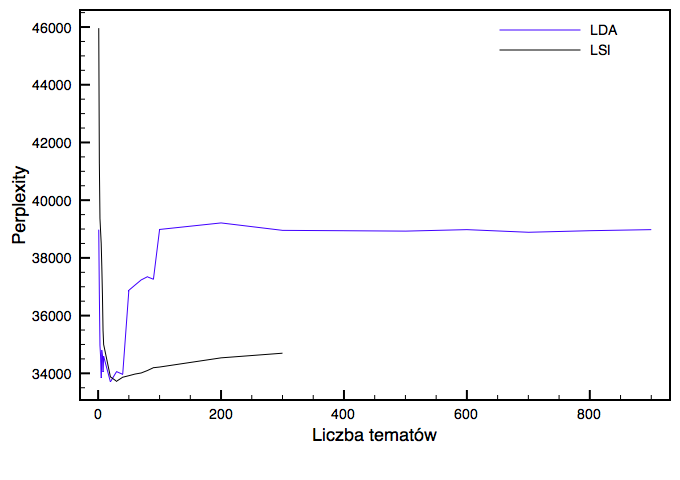
\includegraphics[width=\linewidth]{gfx/perplexity.png}
\label{fig:perplexity}
\end{figure}

\FloatBarrier

\subsection{Wnioski}

Algorytm LDA daje gorszej jakości (a przynajmniej mniej stabilne) wyniki dla
typowych problemów klasyfikacji i wyszukiwania informacji spotykanych w
codziennej praktyce. Wydaje się za to być w stanie działać w sytuacji, gdy
wiele różnych tokenów oznacza to samo (przypadek bez wykorzystania stemmingu),
w odróżnieniu od LSI, którego wyniki są wtedy całkowicie nieprzydatne. To
bardzo porządana cecha w przypadku braku odpowiedniego słownika fleksyjnego dla
danego języka.

Przewagą LDA wydaje się być jakość generowanych tematów --- przez wymuszenie
dodatnich wag otrzymujemy na najbardziej znaczących pozycjach (z najwyższymi
wagami) słowa opisujące dany dokument/temat, podczas gdy w przypadku LSI mogą
to być słowa najodleglejsze. Takie zachowanie może okazać się korzystne w
zastosowaniach typu tagowanie dokumentów lub automatyczne generowanie
podsumowań czy słów kluczowych.

\section{Podsumowanie}

\bibliographystyle{abbrv}
\bibliography{thesis}

\enddocument
